\chapter{Background}\label{chapter:background}

Software testing aims to uncover inputs that cause a program to behave
incorrectly or enter an unsafe state. Fuzzing automates this search by
repeatedly executing a program with generated inputs and using observations from
these executions to guide further input generation. Despite their effectiveness,
fuzzing campaigns can require substantial computational resources and
considerable effort to explore code unrelated to the behavior of interest. This
chapter introduces the foundations required to understand the approach presented
in this thesis. It first discusses greybox fuzzing and the role of seed corpora,
then considers regressions and the identification of change-affected code
through program slicing. Finally, it introduces large language models and their
application to software testing and agentic input generation.

\section{Greybox Fuzzing and Seed Corpora}
\label{sec:greybox}

Fuzzing has become a dominant automated approach to software vulnerability
discovery~\cite{manesArtScienceEngineering2019}, both in the literature and in
deployment: OSS-Fuzz alone has found over 20 thousand bugs across hundreds of
open-source projects~\cite{dingEmpiricalStudyOSSFuzz2021}.

\paragraph{Input Generation Strategies.}
At a high level, fuzzing is the process of repeatedly executing a program with
generated inputs, potentially malformed, to trigger bugs. Inputs should
generally remain sufficiently close to structurally valid inputs; otherwise, the
core logic of the \ac{SUT} may never be reached. These inputs can either be
constructed from scratch using a model of the input format
(\emph{generation-based} fuzzing) or derived by semi-randomly perturbing
existing semi-valid inputs referred to as \emph{seeds} (\emph{mutation-based} fuzzing). 
Fuzzing can further be classified according to the fuzzer's knowledge of the
\ac{SUT}:

\begin{description}
  \item[White-box] The fuzzer performs a detailed analysis of the program.
  \item[Black-box] The fuzzer only observes the externally visible outcome of
    an input.
  \item[Grey-box] The fuzzer lies between these two extremes: rather than
    reasoning about the program's semantics, it observes execution through
    lightweight instrumentation.
\end{description}

Greybox fuzzing thus provides more feedback than black-box fuzzing while
avoiding the computational cost of detailed white-box analysis.

\paragraph{Coverage-guided Greybox Fuzzing.}
AFL~\cite{zalewski2017american} by Zalewski is one of the most influential greybox
mutation-based fuzzers, and the continuation of it is called
AFL++~\cite{fioraldiAFLCombiningIncremental2020} is deemed to be the de facto standard for fuzzing. AFL introduced coverage-guided
greybox fuzzing, using code coverage as a feedback signal to guide mutation. The
\ac{SUT} is instrumented to record which branching sections of the code, also
referred to as \emph{edges}, are executed. After each execution, the fuzzer
observes the covered edges and whether the execution resulted in a crash. AFL
uses this information to determine whether a mutation is interesting, for
example, because it reaches previously unseen edges, in which case the resulting
input is added to the corpus.

\paragraph{Campaign Cost.}
Although this lightweight instrumentation is very efficient and
allowing the fuzzer to spend most of its computational resources on executing
numerous inputs against the \ac{SUT}, mutation-based fuzzing can
require substantial time and computational resources to trigger a particular
bug. Fuzzer evaluations are therefore recommended to run for at least
12--24~h~\cite{kleesEvaluatingFuzzTesting2018,
bohmeReliabilityCoveragebasedFuzzer2022, schloegelSoKPrudentEvaluation2024},
while deployments such as OSS-Fuzz fuzz targets continuously and
indefinitely~\cite{serebryanyOSSFuzzGooglesContinuous2017}. Returns nonetheless
diminish as coverage approaches a plateau~\cite{dingEmpiricalStudyOSSFuzz2021},
making the efficiency of individual fuzzing campaigns an important concern.

\paragraph{Time to Exposure.}
A natural metric for this concern is the \acf{TTE}: the wall-clock time required
for a campaign to trigger a given bug. Since fuzzing is a randomized search
process, \ac{TTE} is not a fixed property of a target, but a distribution over
campaigns, and is therefore typically measured across repeated
runs~\cite{kleesEvaluatingFuzzTesting2018}. Reducing \ac{TTE} is a central goal
of work improving greybox fuzzing, either by refining the feedback
signal~\cite{ganCollAFLPathSensitive2018,bohmeBoostingFuzzerEfficiency2020} or by
improving the mutation engine~\cite{lyuMOPTOptimizedMutation2019,
aschermannREDQUEENFuzzingInputtoState2019}. An orthogonal approach is to improve
the inputs the fuzzer starts with: the seed corpus. The initial corpus serves as
the basis for subsequent mutation and can substantially influence the outcome of
a fuzzing campaign~\cite{kleesEvaluatingFuzzTesting2018,
herreraSeedSelectionSuccessful2021}.

\paragraph{What Makes a Good Seed Corpus.}
What constitutes a good seed corpus is less settled. One motivation for
considering initial code coverage is that a more comprehensive corpus may reduce
the amount of exploration needed to reach relevant program regions. However,
empirical evidence does not establish a simple relationship between corpus
coverage and fuzzing performance. Herrera~et~al.~\cite{herreraSeedSelectionSuccessful2021}
report that seed selection has a substantial effect on campaign outcomes, but
not a monotonic one, with minimal seed sets remaining competitive on several
targets. Independent of coverage, a corpus should be minimal in both set size
and individual seed size to reduce I/O overhead and the mutation space explored
for each seed. An existing corpus can therefore be improved by removing or
combining redundant seeds that cover similar code regions, a process known as
\emph{corpus distillation}~\cite{rebertOptimizingSeedSelection}.

\bigskip
Our work combines corpus distillation with seed augmentation. We first distill
an existing corpus, then augment it by generating additional seeds to cover
missing or relevant regions of the program, thereby preserving the information
already encoded in the corpus. Unlike approaches that aim to maximize coverage
of the entire program, we focus on seed generation on code affected by a recent
change to identify bugs known as \emph{regressions}.

\section{Regressions and Change-Affected Code}
\label{sec:regressions}

Software is developed incrementally, and each change carries the risk of
breaking previously correct behavior. A \emph{regression} is a fault introduced
by a software change that causes previously correct behavior to become
incorrect~\cite{avizienisBasicConceptsTaxonomy2004}. Regression testing is
therefore inherently change-focused: rather than treating the program as a
uniform search space, it concentrates testing effort on behavior that may have
been affected by a modification. Making this intuition operational requires
answering two questions:

\begin{description}
  \item[Fault proneness.] Is changed code indeed associated with a substantial
    proportion of faults?
  \item[Scope of a change.] What precisely constitutes code affected by a
    change?
\end{description}

\paragraph{Changed code is disproportionately fault-prone.}
This has long been observed in the defect-prediction literature, where measures
of code churn relative to component size can predict defect
density~\cite{nagappanUseRelativeCode2005}. It also holds specifically for bugs
found through fuzzing: in an empirical study of fuzzer-generated bug reports in
OSS-Fuzz, Zhu and Böhme found that 77\% of 23{,}000 bugs were
regressions~\cite{zhuRegressionGreyboxFuzzing2021b}. The proportion increases as
a project matures: the probability that a report is a regression rises from 20\%
for a project's first bug to 92\% after a few hundred reports, while most code
is never changed.

% ---------------------------------------------------------------
%  curl commit dd7521b.  Line numbers verified against
%  lib/transfer.c and lib/curl_ctype.h at that commit.
%  Panel (a) is wrapped in a save box and shrunk only if it would
%  overflow, so it can never run into panel (b).
%  In a two-column paper use figure* instead of figure.
% ---------------------------------------------------------------
\usetikzlibrary{positioning,arrows.meta,calc,shapes.geometric,shapes.misc,fit,backgrounds}
 
\definecolor{diffadd}{HTML}{CCEFCC}
\definecolor{diffaddtext}{HTML}{176117}
\definecolor{diffdel}{HTML}{F7D4D4}
\definecolor{diffdeltext}{HTML}{9B1111}
\definecolor{crashbg}{HTML}{FFE3B8}
\definecolor{crashfg}{HTML}{9A5300}
\definecolor{sizebg}{HTML}{E6E6E6}
\definecolor{sizefg}{HTML}{4A4A4A}
\definecolor{macrobg}{HTML}{E4E9F2}
\definecolor{macrofg}{HTML}{2E3F5C}
\definecolor{ctrlblue}{HTML}{15507F}
\definecolor{datapurple}{HTML}{6A3D9A}
 
\lstdefinestyle{pdgfig}{
  language=C, basicstyle=\ttfamily\scriptsize,
  keywordstyle=\color{black}, commentstyle=\color{black!45}\itshape,
  stringstyle=\color{black!70}, columns=fullflexible, keepspaces=true,
  showstringspaces=false, numbers=none, escapeinside={(*@}{@*)},
  xleftmargin=0pt, aboveskip=2pt, belowskip=2pt,
}
 
\tikzset{
  box/.style ={draw=black!60, rounded corners=2pt, fill=black!4,
               font=\scriptsize\ttfamily, align=center, inner sep=4pt,
               minimum height=7mm, text width=26mm},
  sml/.style ={box, text width=22mm},
  pred/.style={shape=chamfered rectangle, rounded corners=0pt,
               chamfered rectangle xsep=1em, chamfered rectangle angle=45},
  chg/.style ={box, draw=diffaddtext, line width=0.9pt, fill=diffadd},
  crs/.style ={box, draw=crashfg,     line width=0.9pt, fill=crashbg},
  siz/.style ={box, draw=sizefg, line width=0.8pt, fill=sizebg},
  mac/.style ={box, draw=macrofg, line width=0.8pt, fill=macrobg},
  src/.style ={box, draw=black!55, fill=white},
  phi/.style ={draw=black!60, fill=black!6, ellipse, inner sep=2pt,
               font=\scriptsize},
  cf/.style  ={-{Latex[length=1.8mm]}, ctrlblue, semithick},
  df/.style  ={-{Latex[length=1.8mm]}, datapurple, semithick,
               dash pattern=on 2.2pt off 1.8pt},
  fd/.style  ={-{Latex[length=2.4mm]}, crashfg, line width=1.1pt,
               dash pattern=on 3.5pt off 2pt},
  mx/.style  ={-{Latex[length=1.8mm]}, macrofg, dotted, thick},
  mis/.style ={{Latex[length=2.4mm]}-{Latex[length=2.4mm]}, crashfg,
               line width=1.1pt, dash pattern=on 3pt off 2pt},
  slice/.style={draw=black!70, line width=0.9pt, rounded corners=4pt,
               dash pattern=on 3pt off 1.6pt on 0.8pt off 1.6pt,
               fill=yellow!35, inner sep=2.6pt},
  lb/.style  ={font=\tiny\sffamily, inner sep=1.5pt, fill=white,
               fill opacity=0.9, text opacity=1},
}
 
% line-number label: smaller and quieter than the code it annotates
\newcommand{\lno}[1]{{\tiny\sffamily\textcolor{black!50}{#1}}}
\newsavebox{\pdgcode}
\newlength{\pdgw}
% width of the longest listing line (48 monospace chars) plus colorbox padding
\settowidth{\pdgw}{\ttfamily\scriptsize 123456789012345678901234567890123456789012345678}
\addtolength{\pdgw}{10pt}
 
% ---- panel (a) is measured first, then shrunk only if too wide ----
\begin{lrbox}{\pdgcode}
\begin{minipage}{\pdgw}
\begin{lstlisting}[style=pdgfig]
(*@\textcolor{black!45}{\itshape lib/curl\_ctype.h}@*)
  68(*@\colorbox{macrobg}{\texttt{~\#define ISPRINT(x) \textbackslash}}@*)
   (*@\colorbox{macrobg}{\texttt{~~(Curl\_isprint((int)((unsigned char)x)))}}@*)
 
(*@\textcolor{black!45}{\itshape lib/transfer.c -- strlen\_url(), unchanged}@*)
1477(*@\colorbox{sizebg}{\texttt{~~~if(*ptr >= 0x80)}}@*)
1478(*@\colorbox{sizebg}{\texttt{~~~~~newlen += 2;}}@*)
1479(*@\colorbox{sizebg}{\texttt{~~~newlen++;}}@*)
 
(*@\textcolor{black!45}{\itshape lib/transfer.c -- caller, unchanged}@*)
1780   newlen = strlen_url(newurl, FALSE);
1785   newest = malloc(newlen + 1);
1789   strcpy_url(newest, newurl, FALSE);
 
(*@\textcolor{black!45}{\itshape lib/transfer.c -- strcpy\_url(), changed}@*)
1500   char *optr = output;
1508   for(iptr = (unsigned char *)url;
1509       *iptr;
1510       iptr++) {
1517     switch(*iptr) {
1518     case '?': ...
1521     default:
1522(*@\colorbox{diffdel}{\textcolor{diffdeltext}{\texttt{-~~~~~~if(*iptr >= 0x80) \{}}}@*)
1522(*@\colorbox{diffadd}{\textcolor{diffaddtext}{\texttt{+~~~~~~if(!ISPRINT(*iptr)) \{}}}@*)
1523         snprintf(optr,4,"%%%02x",*iptr);
1524         optr += 3;
1525       }
1526       else
1527         *optr++=*iptr;
1528       break;
1529     case ' ': ...
1538     }
1539   }
1540(*@\colorbox{crashbg}{\texttt{~~*optr = 0;}}@*)
\end{lstlisting}
\end{minipage}
\end{lrbox}
 
\begin{figure}[tb]
\centering
\begin{minipage}[t]{0.44\linewidth}
\centering
{\footnotesize\textbf{(a) reference code (commit \texttt{dd7521b})}}\\[3pt]
\ifdim\wd\pdgcode>\linewidth
  \resizebox{\linewidth}{!}{\usebox{\pdgcode}}%
\else
  \usebox{\pdgcode}%
\fi
\vspace{3pt}
 
{\tiny\sffamily
 \colorbox{macrobg}{\vphantom{Ay}~~}~macro \;
 \colorbox{sizebg}{\vphantom{Ay}~~}~sizing \;
 \colorbox{diffdel}{\vphantom{Ay}~~}~removed \;
 \colorbox{diffadd}{\vphantom{Ay}~~}~added \;
 \colorbox{crashbg}{\vphantom{Ay}~~}~faulting}
\end{minipage}
\hfill
\begin{minipage}[t]{0.53\linewidth}
\centering
{\footnotesize\textbf{(b) control- and data-flow dependences}}\\[3pt]
\resizebox{\linewidth}{!}{%
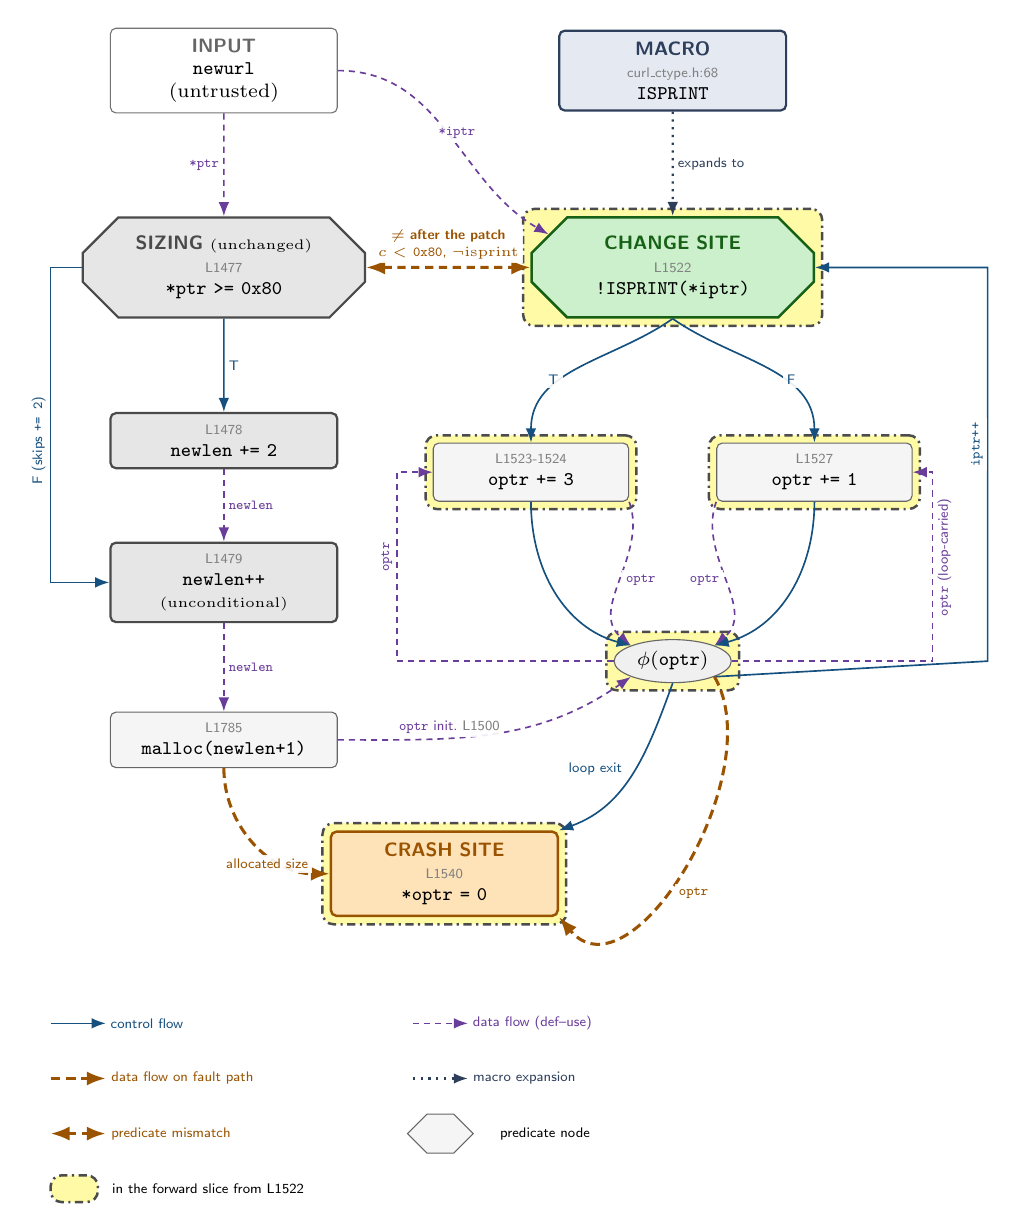
\begin{tikzpicture}
 
\node[src] (url) at (-3.1,2.5)
  {\textcolor{black!60}{\sffamily\bfseries INPUT}\\ \texttt{newurl}\\
   \textrm{\scriptsize(untrusted)}};
 
\node[mac] (mac) at (2.6,2.5)
  {\textcolor{macrofg}{\sffamily\bfseries MACRO}\\ \lno{curl\_ctype.h:68}\\ \texttt{ISPRINT}};
 
\node[siz,pred] (sizep) at (-3.1,0)
  {\textcolor{sizefg}{\sffamily\bfseries SIZING}~\textrm{\tiny(unchanged)}\\
   \lno{L1477}\\ \texttt{*ptr >= 0x80}};
 
\node[chg,pred] (writep) at (2.6,0)
  {\textcolor{diffaddtext}{\sffamily\bfseries CHANGE SITE}\\ \lno{L1522}\\
   \texttt{!ISPRINT(*iptr)}};
 
\node[siz] (sdefa) at (-3.1,-2.2) {\lno{L1478}\\ \texttt{newlen += 2}};
\node[siz] (sdefb) at (-3.1,-4.0)
  {\lno{L1479}\\ \texttt{newlen++}\\ \textrm{\tiny(unconditional)}};
 
\node[sml] (esc) at (0.8,-2.6) {\lno{L1523-1524}\\ \texttt{optr += 3}};
\node[sml] (cpy) at (4.4,-2.6) {\lno{L1527}\\ \texttt{optr += 1}};
 
\node[box] (alloc) at (-3.1,-6.0) {\lno{L1785}\\ \texttt{malloc(newlen+1)}};
 
\node[phi] (phi) at (2.6,-5.0) {$\phi(\texttt{optr})$};
 
\node[crs] (crash) at (-0.3,-7.7)
  {\textcolor{crashfg}{\sffamily\bfseries CRASH SITE}\\ \lno{L1540}\\ \texttt{*optr = 0}};
 
% ---- forward slice from the change site (background layer) ----
\begin{scope}[on background layer]
  \foreach \n in {writep,esc,cpy,phi,crash}{\node[slice, fit=(\n)]{};}
\end{scope}
 
% ---- data flow (def-use) ----
\draw[df] (url) -- node[lb,midway,left]{\texttt{*ptr}} (sizep);
\draw[df] (url.east) to[out=0,in=150]
      node[lb,pos=.55,above]{\texttt{*iptr}} (writep.north west);
\draw[df] (sdefa) -- node[lb,midway,right]{\texttt{newlen}} (sdefb);
\draw[df] (sdefb) -- node[lb,midway,right]{\texttt{newlen}} (alloc);
\draw[df] (alloc.east) to[out=0,in=215]
      node[lb,pos=.35,above]{\texttt{optr} init.\ \lno{L1500}} (phi.south west);
 
% optr defined at both branches, reaching the merge
\draw[df] (esc.south east) to[out=290,in=140]
      node[lb,pos=.5,right]{\texttt{optr}} (phi.north west);
\draw[df] (cpy.south west) to[out=250,in=40]
      node[lb,pos=.5,left]{\texttt{optr}} (phi.north east);
 
% loop-carried: merged value read again by both branches next iteration
\draw[df] (phi.west) -- (-0.9,-5.0) -- (-0.9,-2.6)
      node[lb,pos=.55,rotate=90,above]{\texttt{optr}} -- (esc.west);
\draw[df] (phi.east) -- (5.9,-5.0) -- (5.9,-2.6)
      node[lb,pos=.55,rotate=90,below]{\texttt{optr} (loop-carried)} -- (cpy.east);
 
% ---- macro expansion ----
\draw[mx] (mac) -- node[lb,midway,right]{expands to} (writep);
 
% ---- control flow ----
\draw[cf] (sizep) -- node[lb,midway,right]{T} (sdefa);
\draw[cf] (sizep.west) -- (-5.3,0) -- (-5.3,-4.0)
      node[lb,pos=.55,rotate=90,above]{F (skips \texttt{+= 2})} -- (sdefb.west);
\draw[cf] (writep.south) to[out=215,in=90] node[lb,pos=.6,left]{T} (esc.north);
\draw[cf] (writep.south) to[out=325,in=90] node[lb,pos=.6,right]{F} (cpy.north);
\draw[cf] (esc.south) to[out=270,in=165] (phi.north west);
\draw[cf] (cpy.south) to[out=270,in=15]  (phi.north east);
\draw[cf] (phi.south east) -- (6.6,-5.0) -- (6.6,0)
      node[lb,pos=.55,rotate=90,above]{\texttt{iptr++}} -- (writep.east);
\draw[cf] (phi.south) to[out=250,in=20]
      node[lb,pos=.55,above left]{loop exit} (crash.north east);
 
% ---- the two predicates no longer agree ----
\draw[mis] (sizep) -- node[lb,midway,above,align=center,yshift=1pt]
      {$\neq$ \textbf{after the patch}\\ $c<\texttt{0x80}$, $\neg\mathrm{isprint}$}
      (writep);
 
% ---- data flow along the fault path ----
\draw[fd] (alloc.south) to[out=270,in=180]
      node[lb,pos=.6,below]{allocated size} (crash.west);
\draw[fd] (phi.south east) to[out=300,in=310]
      node[lb,pos=.55,below right]{\texttt{optr}} (crash.south east);
 
\begin{scope}[shift={(-5.3,-9.6)}]
  \draw[cf] (0,0)    -- (0.7,0)    node[lb,right]{control flow};
  \draw[df] (4.6,0)  -- (5.3,0)    node[lb,right]{data flow (def--use)};
  \draw[fd] (0,-0.7) -- (0.7,-0.7) node[lb,right]{data flow on fault path};
  \draw[mx] (4.6,-0.7)--(5.3,-0.7) node[lb,right]{macro expansion};
  \draw[mis](0,-1.4) -- (0.7,-1.4) node[lb,right]{predicate mismatch};
  \node[pred, draw=black!60, fill=black!4, font=\tiny,
        inner sep=2pt, text width=4mm, align=center]
        at (4.95,-1.4) {\vphantom{Ay}};
  \node[lb,right] at (5.65,-1.4) {predicate node};
  \node[slice, minimum width=6mm, minimum height=3.4mm, inner sep=0pt]
        at (0.3,-2.1) {};
  \node[lb,right] at (0.72,-2.1) {in the forward slice from L1522};
\end{scope}
 
\end{tikzpicture}}
\end{minipage}
 
\caption{Illustration of a regression in curl that manifests outside the changed code.}
\label{fig:pdg}
\end{figure}

\paragraph{Effects Manifest Beyond the Changed Lines.}
Concentrating effort on changed code is therefore attractive, but the changed
lines themselves are frequently not where a regression manifests. A single
modified statement can influence behavior at locations far from the change. For
example, if a commit alters an array index, subsequent accesses using that index
may be affected, resulting in an out-of-bounds error that may manifest later in
the program. Xiang~et~al.~\cite{xiangCriticalCodeGuided2024} quantify this for
commit-introduced bugs in real-world C programs, finding that the crash site
differs from the change site in over half of the cases they study. For instance,
\Cref{fig:pdg} shows a curl commit that rewrites a single predicate at
line~1522; the resulting out-of-bounds write manifests eighteen lines later at
line~1540, where the output buffer is terminated.

\paragraph{Change Impact Analysis and Program Slicing.}
Determining which parts of a program a change can affect is therefore a
program-analysis problem in its own right, studied under the heading of change
impact analysis~\cite{kretsouChangeImpactAnalysis2021}. Of the approaches
surveyed there, we follow the dependence-based line, which derives the affected
region from the program's control- and data-flow structure rather than from
version history or coupling metrics.

Its central technique is \emph{program slicing}, which reduces a program to the
parts relevant to a given point of interest, the \emph{slicing criterion}, by
exploiting influences between statements arising from data and control
flow~\cite{weiserProgramSlicing1984}. A statement is \emph{data dependent} on
another if it reads a value defined by the other, and \emph{control dependent}
on a predicate if that predicate determines whether it executes. In
\Cref{fig:pdg}(b), line~1540 is data dependent on the updates to \texttt{optr}
at lines~1524 and~1527, and those statements are in turn control dependent on
the predicate at line~1522.

\paragraph{Forward slicing and the cone of influence.}
The original formulation of program slicing follows these influences backward,
yielding the statements that may influence the slicing criterion. Following the
dependencies forward instead yields the statements that may be influenced by the
criterion~\cite{horwitzInterproceduralSlicingUsing1990}. As Gallagher and
Binkley~\cite{gallagherProgramSlicing2008} observe, taking the change site as
the criterion therefore makes forward slicing a direct means of computing code
affected by a change. We refer to the resulting set as the \acf{CoI}, following
Hundsdorfer~\cite{zotero-item-324}, whose forward static slicer we build on in \Cref{chapter:approach}: the set of program points whose behavior may
be influenced by the change, including locations at which a resulting error may
manifest as a crash.

\paragraph{The Role of Control Dependence.}
Computing the \ac{CoI} requires both data and control dependence. In the
example, the changed predicate reads \texttt{*iptr} but writes no value, so it
has no outgoing data dependence. A forward slice based only on data dependence
would therefore contain line~1522 but would not propagate further. Control
dependence instead connects the predicate to lines~1524 and~1527, from which the
slice follows the loop-carried data dependence on \texttt{optr} to the faulting
write at line~1540. The shaded nodes in \Cref{fig:pdg}(b) mark this
slice. The example illustrates why both types of
dependence are necessary to capture the potential effects of a change.

\paragraph{Safety and Precision.}
Two properties characterize the quality of a slicing technique. A technique is
\emph{safe} if every statement affected by the slicing criterion is contained in
the result, and \emph{precise} to the extent that it contains no statements that
are not affected~\cite{alomariSrcSliceVeryEfficient2014}. Both properties matter
in this setting: an unsafe result may omit the code in which a regression
manifests, while an imprecise result may include code unrelated to the change.

\paragraph{Size of the Cone of Influence.}
In practice, the resulting \ac{CoI} can encompass a substantial portion of a
program. Because dependence is transitive, the forward closure can grow with
each dependency step. Across 17 open-source C and C++ projects,
Hundsdorfer~\cite{zotero-item-324} reports that the \ac{CoI} contains 62.19\% of
all basic blocks on average. Thus, they implemented various policies to limit the size of the \ac{CoI}; for example, one can configure it to include slices that are at most 10 basic blocks away from the change site. These sacrifices in safety can significantly reduce the search space; a tradeoff we investigate in \cref{chapter:evaluation}.

\bigskip
In summary, regressions constitute the primary class of bugs identified through fuzzing, yet
their effects often manifest beyond the lines directly modified by a commit.
Forward slicing provides a safe and precise means of identifying the broader region of code that may be affected by a change. This information can be used to focus seed
generation on inputs that can reach and exercise the altered behavior. However,
reaching such code may require satisfying semantic constraints that conventional
mutation-based fuzzers struggle to discover efficiently. Large language models
offer a complementary capability: by leveraging their learned knowledge of
program structure and semantics, they can reason about the input conditions
required to reach the relevant code and generate seeds that provide the fuzzer with
a head start in exploring change-affected behavior.

\section{Large Language Models}
\label{sec:llms}

The rapid advancement of \acp{LLM} has enabled new approaches to automated
program analysis and input generation. Unlike traditional syntactic generators,
\acp{LLM} can leverage knowledge acquired from large-scale pre-training to
generate context-dependent outputs, making them promising for tasks where
syntactic validity alone is insufficient.

\paragraph{LLMs, tokens, and context.}
At their core, \acp{LLM} are autoregressive models that predict the next output
given a sequence of preceding inputs~\cite{brownLanguageModelsAre2020}. Inputs
and outputs are represented as sequences of \emph{tokens}, sub-word units
produced by the model's tokenizer, which also commonly serve as the unit of
measurement and billing for \ac{API} usage. Consequently, the cost of an
experiment is naturally expressed as a \emph{token budget}, and cost per token
is the relevant price metric when comparing models. The amount of information
processed in a single interaction is bounded by the model's \emph{context
window}, the maximum number of tokens the model can attend to at once. Anything
that must inform a generation (source code, tool output, prior reasoning) has
to fit within this bound, which is the primary constraint on how much program
context can be supplied at once.

\paragraph{Decoding parameters.}
At each step, the model produces a probability distribution over the vocabulary,
from which the next token is drawn. Two parameters commonly control this
sampling. The \emph{temperature} rescales the distribution before sampling:
values below \num{1.0} sharpen it towards the most likely token and approach
greedy decoding at \num{0}, while values at or above \num{1.0} preserve or
flatten it, admitting less likely continuations. \emph{Top-$p$}, or nucleus
sampling~\cite{holtzmanCuriousCaseNeural2020}, restricts sampling to the
smallest set of tokens whose cumulative probability mass exceeds $p$, truncating
the long tail of implausible tokens. Higher temperature and higher top-$p$ thus
increase output diversity at the cost of reliability. Because sampling is
stochastic, repeated invocations with identical inputs need not produce
identical outputs, which is why generation experiments are repeated across
multiple runs rather than evaluated from a single sample.

\paragraph{Reasoning about code.}
A key property of \acp{LLM} for software engineering is their ability to
leverage semantic and structural relationships in source code. Recent
evaluations demonstrate that \acp{LLM} can reason about program behavior,
including predicting program outputs and inferring inputs that produce given
outputs~\cite{guCRUXEvalBenchmarkCode2024}. These capabilities have motivated
extensive research into the application of \acp{LLM} to software testing,
including test-case generation, program repair, and
fuzzing~\cite{wangSoftwareTestingLarge2024}. In particular, \acp{LLM} can
complement conventional input-generation techniques by using information about
program structure and semantics to generate inputs that satisfy constraints that
may be difficult to discover through syntactic mutation alone.

\paragraph{Relevance to fuzzing.}
This capability is particularly relevant to fuzzing, where reaching deeper
program logic often requires inputs to satisfy a sequence of semantic conditions
or structural constraints. Recent approaches such as
Cleverest~\cite{liuEvaluatingLLMBasedRegression} demonstrate the potential of
using \acp{LLM} to generate and mutate fuzzing inputs across different target
languages and systems. Rather than replacing traditional fuzzing entirely,
LLM-based generation can provide inputs that give subsequent fuzzing exploration
a more informed starting point.

\paragraph{Agentic generation loops.}
Beyond one-shot generation, an \ac{LLM} can be embedded in an agentic control
loop that combines the model with external tools and execution feedback. A
software harness manages state, invokes tools such as compilers and testing
infrastructure, and returns their results to the model. In approaches such as
ReAct~\cite{yaoReActSynergizingReasoning2023}, the model iteratively selects
actions based on observations from previous actions. This allows generated
inputs to be evaluated and subsequently refined rather than requiring useful
inputs to be produced in a single generation step.

\bigskip
In this work, we combine these capabilities with change-impact information
obtained through forward slicing. The slice identifies the code that may be
affected by a commit, thereby defining the region the generated seeds should
target. The \ac{LLM} uses the affected code and its surrounding context to infer
the input structure and semantic conditions required to reach and exercise this
behavior. The resulting seeds provide a head start for subsequent fuzzing,
combining the semantic and contextual capabilities of the \ac{LLM} with the
fuzzer's scalable exploration.